
\section{LFC photon count errors}\label{appendix:LFC_errors}

\begin{figure}[ht]
    \centering
    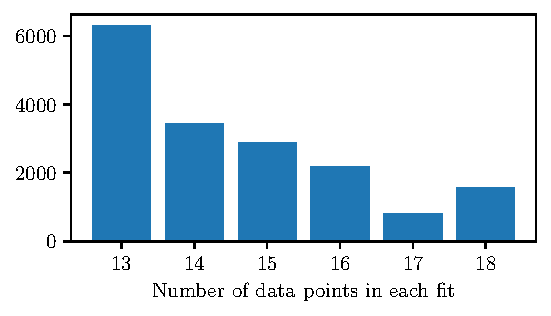
\includegraphics[scale=0.80]{figures/N_data_points.pdf}
    \caption{Number of data points in each LFC peak fit, determined by the average distance between peaks in each order.}
    \label{fig:N_data_points}
\end{figure}

\begin{figure}[ht]
    \centering
    % 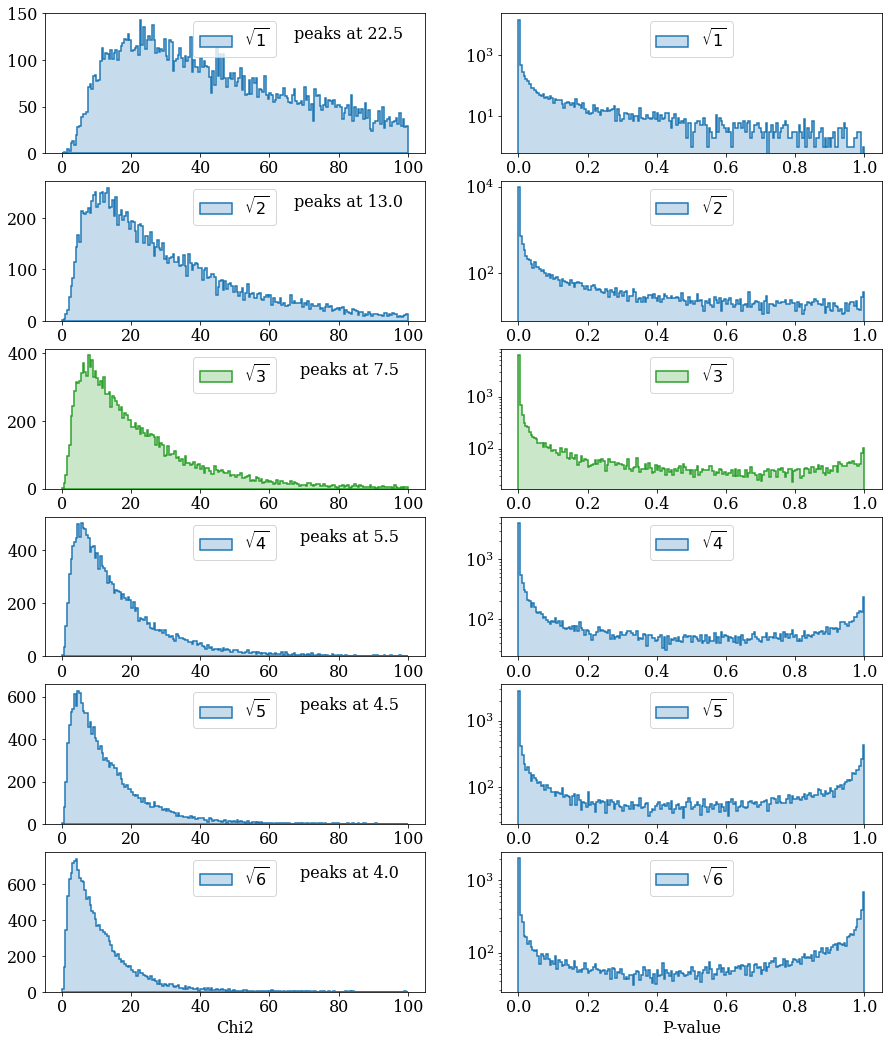
\includegraphics[scale=0.50]{figures/calib_errors_extensive.png}
    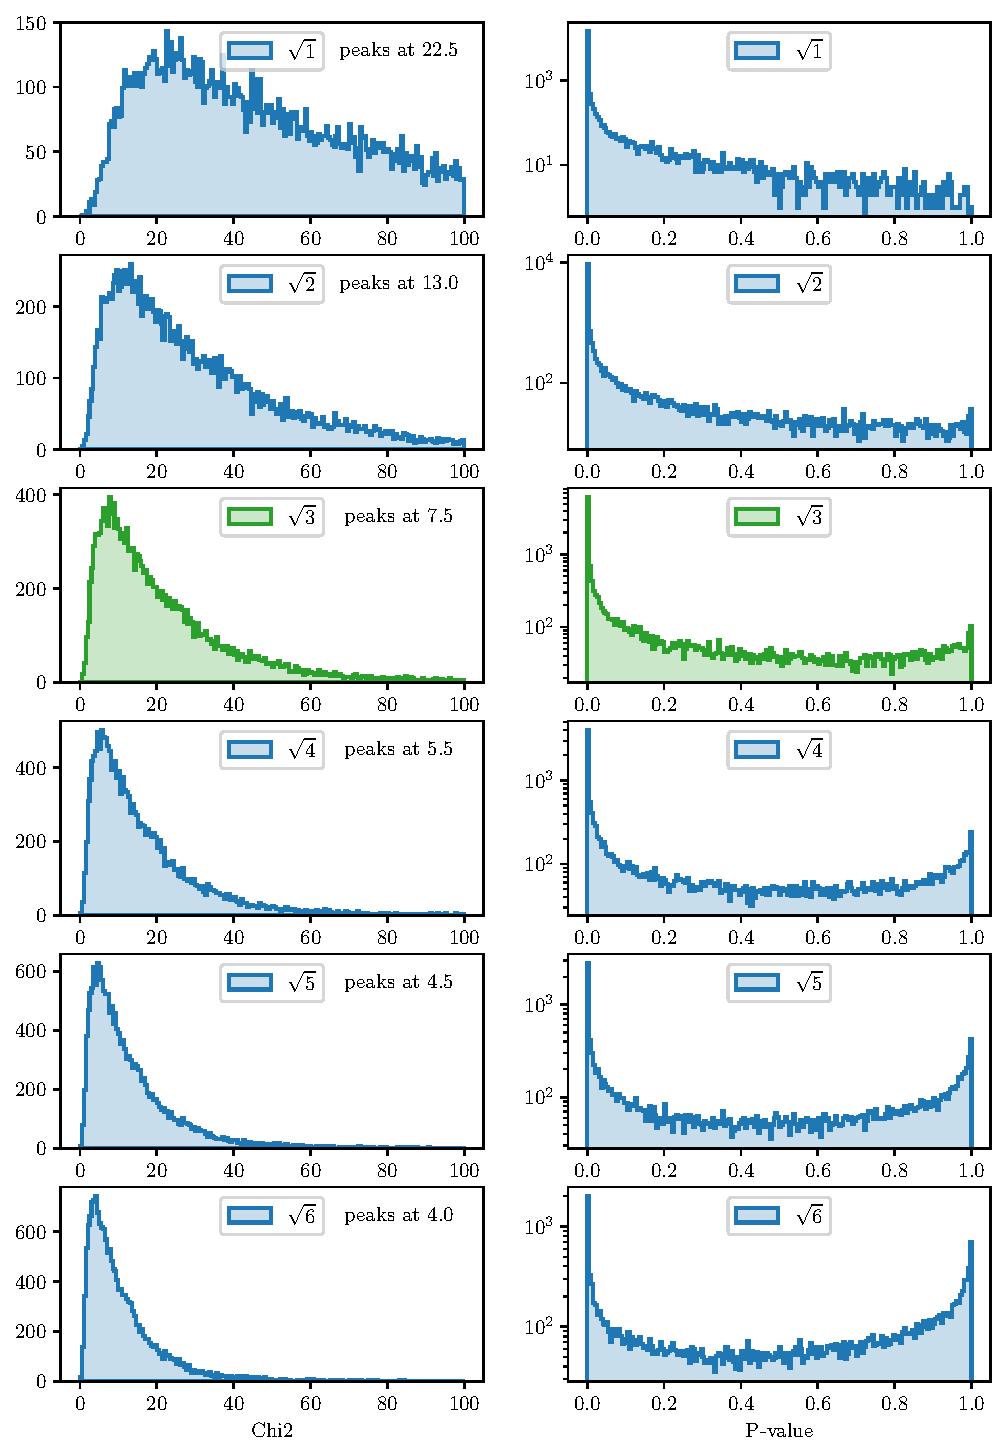
\includegraphics[scale=0.80]{figures/calib_errors_extensive.pdf}
    \caption{Chi2-values and P-values from individual LFC peak super-gauss fits with photon count (spectrum) errors multiplied by different scale-factors.}
    \label{fig:calib_errors_extensive}
\end{figure}


